\subsection{Implementierung der Multi-Level-Monte-Carlo-Methode}
Meinem Programm wird ein Vektor $n$ einer bestimmen L"ange $L$ "ubergeben. Diese L"ange $L$ entspricht der Anzahl der Level. $n(i)$ ist die Anzahl an Samples im jeweiligen Level $i$.
In folgenden Tabellen sind die Ergebnisse f"ur unterschiedliche $\lambda$ und zugeh"origem Vektor $n$ eingetragen. Es ist wieder zu erkennen, dass das Ergebnis stark von der Anzahl der Samples und Level abh"angt. In diesem Kapitel habe ich nur zuf"allig eine Levelanzahl und die zugeh"origen Sampleanzahlen gew"ahlt, um erste Ergebnisse zu sehen. Nat"urlich unter der Voraussetzung, dass die Sampleanzahl mit steigendem Level sinkt. Sp"ater wird dies organisierter geschehen. \\[0.5cm]

 $n=[2000,1000,700,600,500,400,300,100,50]$, Anzahl Level = 9:
\begin{center}
\begin{tabular}{l|c|c|c|c|c|c|c|r}
 $\lambda$&0& $0.1$&$0.2$&$0.3$&$0.5$.&$0.7$&$0.8$&$1$\\
 \hline
 $a(\lambda)$&0   & 0.1329   & 0.1912   & 0.2168  &  0.3605 &   0.4402  &  0.5372  &  0.6495 \\ 
 \hline 
 \end{tabular}
  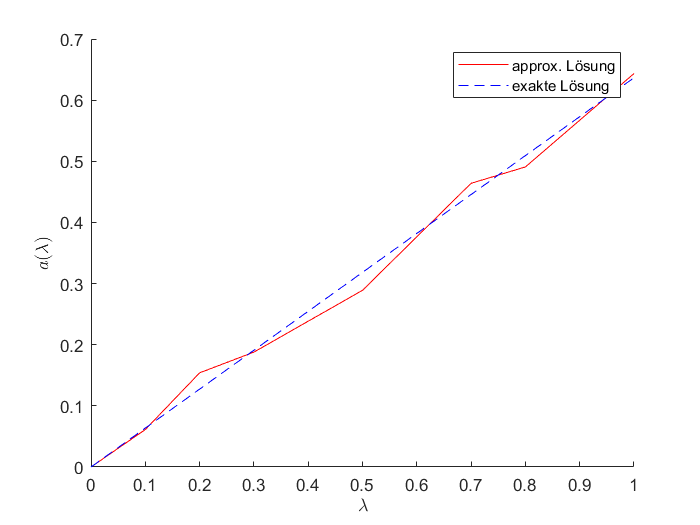
\includegraphics[width=11cm]{MLMC1.png}
 \end{center}\newpage
$n= [5000,4000,3000,2000,1000,700,600,500]$, Anzahl Level = 8,\\
\begin{center}
\begin{tabular}{l|c|c|c|c|c|c|c|r}
 $\lambda$&0& $0.1$&$0.2$&$0.3$&$0.5$.&$0.7$&$0.8$&$1$\\
 \hline
 $a(\lambda)$&0 &   0.0783 &   0.1479 &   0.2261 &   0.3372  &  0.4532  &  0.5229 &   0.6434 \\ 
 \hline 
 \end{tabular}
  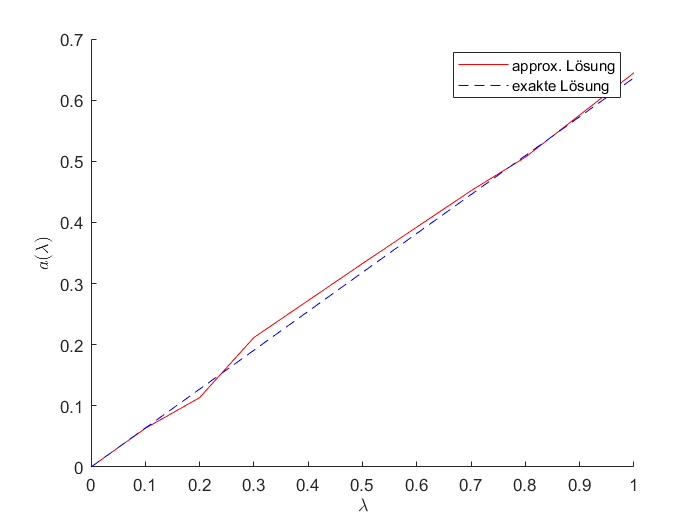
\includegraphics[width=11cm]{MLMC2.png}
 \end{center}
 Das Ergebnis ist trotz kleinerer Levelanzahl besser, da deutlich mehr Samples auf den jeweiligen Leveln genommen wurden.\vspace{0,5cm}
 
$n= [10000,8000,6000,4000,3000,2000,1000,600,500,100,50]$, Anzahl Level = 11:
 \begin{center}
\begin{tabular}{l|c|c|c|c|c|c|c|r}
 $\lambda$&0& $0.1$&$0.2$&$0.3$&$0.5$.&$0.7$&$0.8$&$1$\\
 \hline
 $a(\lambda)$& 0  &  0.0648  &  0.1255 &   0.1935  &  0.3158 &   0.4452 &   0.5074 &   0.6357\\ 
 \hline 
 \end{tabular}
  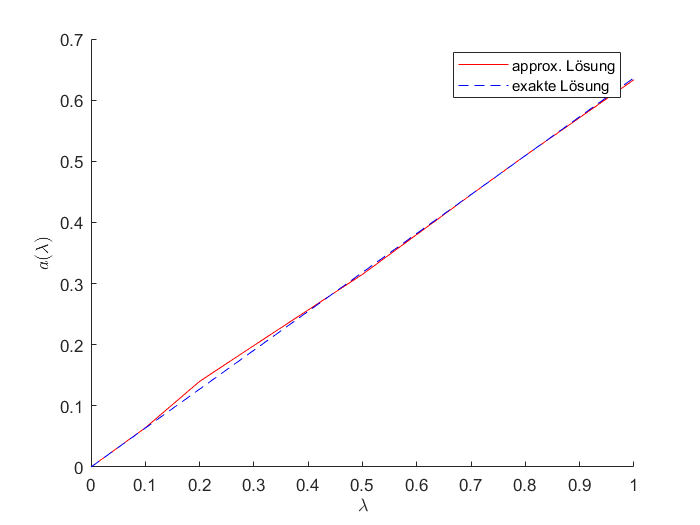
\includegraphics[width=11cm]{MLMC3.png}
 \end{center}\vspace{1cm}

